\section{Prinzipien guten Entwurfs}

Der Abschnitt~\cite[69, 3.7 Prinzipien guten Entwurfs]{Wed09b} vermittelt Kenntnisse, anhand derer man

\begin{itemize}
    \item Kriterien kennt, anhand derer man gute und weniger gute Entwürfe unterscheiden kann
    \item die Güte eines Entwurfs beurteilen kann
    \item besserer Entwürfe erstellen kann
\end{itemize}

\subsection{Was ist ein guter Entwurf}

Die Frage läßt sich nicht generell beantworten, sondern hängt von verschiedenen Faktoren ab, wie den Anforderungen einer konkreten Aufgabe.\\

\subsubsection*{Generelle Prinzipien}

Generelle Prinzipien müssen in allen Entwürfen berücksichtigt werden.
Dazu zählen u.a. \textbf{grundlegende Qualitätsziele} wie

\begin{itemize}
    \item Funktionsfähigkeit
    \item Änderbarkeit
\end{itemize}

\subsection{Teile und Herrsche}
Da Lösungen, die aus einem großen Block bestehen, meist nur schwer nachvollziehbar sind, bietet es sich an, Lösungen in verschiedene Teillösungen aufzuteilen.

\subsubsection*{Vorteile der Zerlegung}

\begin{itemize}
    \item Kleine Teile sind einfacher zu verstehen als große
    \item Änderbarkeit wird erleichtert, da nicht das gesamte System, sondern nur einzelne Teile verstanden werden müssen
    \item Zuverlässigkeit wird erhöht, da Fehler auf Teile begrenzt sind und die Testbarkeit einzelner Teile erleichtert wird, da separat getestet werden kann
    \item gleiche Aufgaben werden in gemeinsamen Teilen gelöst, anstatt gleiche Aufgaben mehrfach in einer Software zu lösen
    \item mehrere Entwickler können gleichzeitig arbeiten
\end{itemize}

\subsubsection*{Nachteile der Zerlegung}
\begin{itemize}
    \item ein System aus sehr vielen kleine Teilen ist schwieriger zu verstehen, weil die Übersicht fehlt
\end{itemize}

\noindent
Dennoch spricht folgendes für eine Zerlegung:

\begin{itemize}
    \item durchgehend einem logischen Entwurf folgen und Entwurfsdokumentation wie Klassendiagramme fördern Verständnis und Übersicht
    \item große Teile sind i.d.R komplizierter aufgebaut, wenn sie stattdessen weiter zerlegt werden könnten
    \item das System ist häufig komplizierter, da komplexe Bausteine wegen interner Komplexität auch komplexere Beziehungen haben
\end{itemize}

\subsubsection*{Beispiel für eine Zerlegung}
\begin{itemize}
    \item Systeme in Subsysteme
    \item Subsysteme in Pakete
    \item Pakete in Klassen
    \item Klassen in Methoden
\end{itemize}


\subsection{Hohe Kohäsion}
Erfolgt eine Zerlegung in Pakete oder Klassen, müssen die einzelnen Teile in einem funktionierenden System so gestaltet sein, dass sie miteinander zusammenarbeiten.\\
Arbeiten Teile miteinander zusammen, hängen sie aber auch in einer bestimmten Art und Weise voneinander ab.\\
Dies wirkt sich auf das Verständnis bzw. Änderung einzelner Teile aus, da dann auch alle zusammenhängenden Teile verstanden bzw. u.U. geändert werden müssen.\\

\noindent
Man nennt diese Art von Abhängigkeit \textbf{Kopplung}.

\subsubsection*{Kopplung vermeiden}
Inwieweit kann man bei stark gekoppelten Teilen noch von einzelnen Teilen sprechen? Kopplung ist also nach Möglichkeit zu vermeiden, um an Ende nicht doch wieder einen stark zusammenhängenden Block zu erhalten, statt ein System aus veilen kleinen Teilen.

\subsubsection*{Erhöhe Zusammenhalt, wo möglich}
Das wichtigste Prinzip lautet:

\blockquote[{\cite[71]{Wed09b}}]{
[\ldots] den Zusammenhalt innerhalb der Teile möglichst hoch zu halten und Abhängigkeiten nach außen zu minimieren (Zusammenhalt = Cohesion).
}
\noindent
Dinge, die zusammengehören, sollen innerhalb eines Teils erledigt werden, anbete Dinge sollten herausgehalten werden, bspw durch:

\begin{itemize}
    \item $\rightarrow$ Operationen, die auf denselben Daten arbeiten, gehören zu einer Klasse
    \item $\rightarrow$ Klassen, die ähnliche Aufgaben haben, liegen in einem Paket
\end{itemize}

\subsubsection*{Typen des Zusammenhalts}

Man unterscheiden zwischen folgenden Typen des Zusammenhalts:

\begin{itemize}
    \item \textbf{Funktionaler Zusammenhalt}
    \item[] ähnliche Funktionalität wird in gleichen Softwareteilen implementiert
    \item[] die Funktionalität ist nach Möglichkeit nicht von anderer Funktionalität abhängig und besitzt keine Nebeneffekte
    \item[] Idealfall: Eine Operation liefert ein bestimmtes Ergebnis und ist unabhängig von vorausgegangen Aufrufen, internen Zuständen oder Teilen des Systems
    \item[] Forderung nach Unabhängigkeit allerdings meist nicht möglich, da in der OO Objekte i.d.R. über Attribute interne Zustände besitzen (s. Abbildung~\ref{fig:adt}); außerdem benutzen Klassen anderen Klassen, oder externe Systeme wie Datenbanken
    \item \textbf{Schichten-Zusammenhalt}
    \item[] Teile, die ähnliche Services für andere Teile zur Verfügung stellen, werden in Schichten zusammengefügt (s. Abschnitt~\ref{sec:architekturmuster})
    \item \textbf{kommunikativer Zusammenhalt}
    \item[] Teile, die auf gleichen Daten operieren, gehören zusammen
    \item[] der Zusammenhalt ist an der Stelle schwächer als der Schichten-Zusammenhalt, da man i.d.R. nicht Geschäftslogik und Zugriff auf Datenbanken in derselben Klasse implementiert, auch, wenn das Model dieselben Daten benötigt
    \item \textbf{Utility-Zusammenhalt}
    \item[] unter ``\textit{Utility}`` werden hier Teile gemeint, die ähnliche Funktionalität bereitstellen, sich aber logisch nicht ordnen lassen (bspw. in Schichten)\footnote{s. bspw. Klassen aus \url{https://docs.oracle.com/en/java/javase/21/docs/api/java.base/java/util/package-summary.html}, abgerufen 19.04.2024}
\end{itemize}

\noindent
Der Zusammenhalt wird in der Reihenfolge schwächer (s. Abbildung~\ref{fig:zusammenhalt}).

\begin{figure}
    \centering
    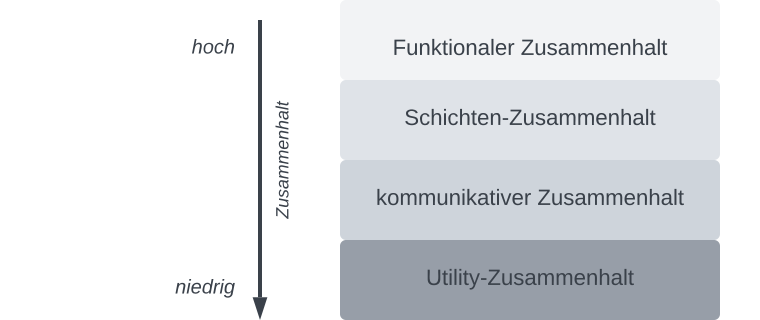
\includegraphics[scale=0.4]{part two/Objektorientierter Entwurf/img/zusammenhalt}
    \caption{Typen des Zusammenhaltes. Der funktionale Zusammenhalt ist verständlicherweise sehr hoch, während der Utility-Zusammenhalt eher schwach ist (Quelle: eigene)}
    \label{fig:zusammenhalt}
\end{figure}


\begin{figure}
    \centering
    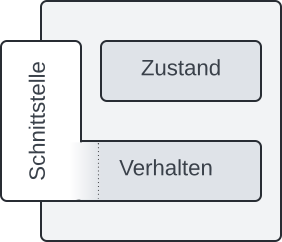
\includegraphics[scale=0.4]{part two/Objektorientierter Entwurf/img/adt}
    \caption{Schematische Darstellung eines abstrakten Datentyps. Verhalten und Zustand sind sowohl intern als auch extern änderbar.  (Quelle: eigene)}
    \label{fig:adt}
\end{figure}

\subsection{Lose Kopplung}
\textbf{Kopplungen} sind unvermeidlich, da bestimmte Teile zusammenarbeiten müssen.\\
Dennoch müssen Kopplungen möglichst schwach sein, da die Teile der Software unabhängig voneinander sein sollen.

\subsubsection*{Typen von Kopplungen}
Im Software Engineering wird die Kopplung von Teilen nach Typen klassifiziert, wobei die Stärke der Kopplung unterschiedlich bewertet wird (s. Abbildung~\ref{fig:kopplung}).

\noindent
Mit absteigender Reihenfolge nimmt auch die Stärke der Kopplung in folgender Liste ab:


\begin{itemize}
    \item \textbf{Content-Kopplung}
    \item[] ein Teil ändert interne Daten eines anderen Teils
    \item[] die ändernde Klasse ist von der Struktur der zu ändernden Klasse \textbf{abhängig}
    \item[] diese Art der Kopplung sollte vermieden werden, bspw. über Zugriffsmodifizierer und Zugriffsmethoden
    \item[] unerwünschte Seiteneffekte können bspw. über das \textit{Immutable}-Pattern\footnote{
    s. Abschnitt~\ref{subsec:immutable}
    } erreicht werden
    \item \textbf{Common-Kopplung}
    \item[] bezeichnet Kopplung über die gemeinsame Verwendung globaler Variablen\footnote{
        bspw. unsachgemäße Verwendung von \textit{static} in Java
    }
    \item[] führt zu unlesbarem und schwer änderbaren Code, und sollte vermieden werden
    \item \textbf{Stamp-Kopplung}
    \item[] ein Objekt wird als Argument einer Methode verwendet
    \item[] wird der öffentliche Teil der Klasse des Objektes geändert, muss auch die aufrufende Methode geändert werden
    \item[] zur vermeidung dieser Kopplung können einfache Variablen übergeben werden\footnote{
        was dann wiederum die \textbf{Data-Kopplung} erhöht, s.u.
    }, oder es werden \textit{Interfaces} oder Klasse genutzt, die weit oben in der Ableitungshierarchie stehen
    \item[] muss man sich für eine Alternative entscheiden, sollte man bedenken, dass die Anzahl der einfachen Variablen nicht zu groß sein darf
    \item \textbf{Data-Kopplung}
    \item[] je mehr Argumente eine Methode hat, desto größer ist die Kopplung mit der benutzenden Komponente\footnote{
    ``The ideal number of arguments for a function is zero (niladic).`` (\cite[40]{Mar08}). Monadische Funktionen sind Funktionen mit einem Argument, dyadische mit zwei, triadische entsprechend mit 3 Argumenten. Polyadische Funktionen sollten laut \textit{Martin} vermieden werden (ebenda).
    }
    \item[] \textbf{Stamp-Kopplung} und \textbf{Data-Kopplung} bedingen sich gegenseitig: Wird Stamp-Kopplung vermieden, erhöht sich i.d.R. Data-Kopplung, und umgekehrt
    \item \textbf{Routine Call-Kopplung}
    \item[] eine Methode ruft eine andere Methode auf
    \item[] werden sehr viele Methode eines anderen Teils aufgerufen, sollte man die Zerlegung überlegen\footnote{
    s. hierzu auch \textbf{Feature Envy}, ein \textit{Code Smell}, der dadurch charakterisiert ist, dass ``a method seems more interested in a class than the one it actually is in`` \cite[80 f.]{Fow99}
    }
    \item[] werden Methoden immer in gleicher Sequenz aufgerufen, könnte man überlegen, die Sequenz auch als eigenständige Methode zusammenfassen
\end{itemize}

\begin{figure}
    \centering
    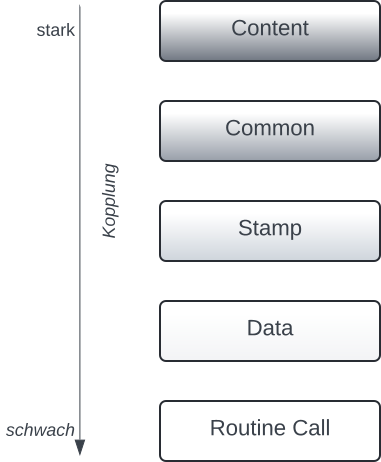
\includegraphics[scale=0.4]{part two/Objektorientierter Entwurf/img/kopplung}
    \caption{Typen von Kopplung, mit absteigender Anordnung werden die Kopplungskonzepte schwächer.  (Quelle: in Anlehnung an \cite[73, Abb. 3.18]{Wed09b})}
    \label{fig:kopplung}
\end{figure}

\subsection{Grundlegende Prinzipien, die weiterhelfen}

\subsubsection*{Abstraktion}
Eine der grundlegenden Prinzipien ist das Prinzip der \textbf{Abstraktion}\footnote{
\textit{Wedemann} merkt an, dass die Bedeutung der Abstraktion für das Software Engineering ``von \textit{Barbara Liskov} und \textit{John Guttag} entdeckt wurde`` (\cite[75, Hervorhebung eigene]{Wed09b}) und erwähnt ein ``sehr anspruchsvolles Buch`` der beiden zu dem Thema, leider ohne weitere Quellenangabe. Man darf vermuten, dass hiermit \cite{LG00} gemeint ist
}.

\noindent
Das Prinzip besagt, dass Bauteile und Abläufe nach außen hin abstrakt sein sollen, also Details weggelassen werden sollten.

\vspace{2mm}
\begin{tcolorbox}[title=Abstraktion]
    \blockquote[{\cite[75, Hervorhebung eigene]{Wed09b}}]{
        Unter \textbf{Abstraktion} versteht man das Herausheben von Wesentlichem, Charakteristischem oder Gesetzmäßigem. Das Prinzip der Abstraktion beruht auf der Beobachtung, dass ein Teil leichter zu verstehen ist, wenn nicht alle Details verstanden werden müssen, sondern nur das Wesentliche.
    }
\end{tcolorbox}
\vspace{2mm}

\subsubsection*{Beispiele für Abstraktion}
\begin{itemize}
    \item Vertikale Schichten sind eine schrittweise Abstraktion von der Hardware
    \item öffentliche Schnittstellen einer Klasse\footnote{
        was als Geheimnisprinzip verstanden werden kann, das \textbf{Content-Kopplung} verhindert
    } können als Abstraktion der Klasse gesehen werden
    \item werden Interfaces zur Vermeidung von \textbf{Stamp-Kopplung} verwendet, ist das Interface die Abstraktion der tatsächlichen Klasse
    \item ein \textbf{Iterator} ist eine Abstraktion des Zugriffs auf eine Datenstruktur
    \item die Ergebnisse von Anforderungen, Analyse und Entwurf können als Abstraktion des zu erstellenden Systems betrachtet werden
\end{itemize}


\susubsection*{The Law of Demeter}
\textit{Lieberherr}, \textit{Holland}, und \textit{Riel} formulieren 1988 in \cite{LHR88} das \textbf{Law of Demeter}, das das Ziel hat, eine Software möglichst modular zu erstellen.
Dabei ist das Prinzip recht einfach gehalten:

\blockquote[{\cite[325]{LHR88}}]{
    Any method written to obey this Law will only know about the immediate structure of the class to which it is attached.
}

\noindent
\textit{Martin} schreibt hierzu:

\blockquote[{\cite[97 f.]{Mar08}}]{
[...] the law of Demeter says that a method $f$ of a class $C$ should only call the methods of these:
\begin{itemize}
    \item $C$
    \item An object created by $f$
    \item An object passed as an argument to $f$
    \item An object held in an instance variable of $C$
\end{itemize}
}
\noindent
und faßt ebenda das Prinzip folgendermaßen zusammen: ``talk to friends, not to strangers.``\footnote{
s. hierzu auch \url{https://www2.ccs.neu.edu/research/demeter/demeter-method/LawOfDemeter/general-formulation.html}, abgerufen 20.04.2024
}

\subsubsection*{Vermeidung zirkulärer Abhängigkeiten}
Eine \textbf{zirkuläre Abhängigkeit} liegt vor, wenn Beziehungen zwischen Klassen kreisförmig sind (s. Abbildung~\ref{fig:zirkulaer} a).\\
Dadurch können Klassen nicht einzeln entwickelt bzw. getestet werden, was eine sehr starke Kopplung ausdrückt.\\
Eine zyklische Abhängigkeit ist lft ein Fehler im Entwurf.\\
Beruht die Abhängigkeit nicht auf einem Fehler, kann sie durch den Einsatz eines Interfaces aufgelöst werden (s. Abbildung~\ref{fig:zirkulaer} b).).

\begin{figure}
    \centering
    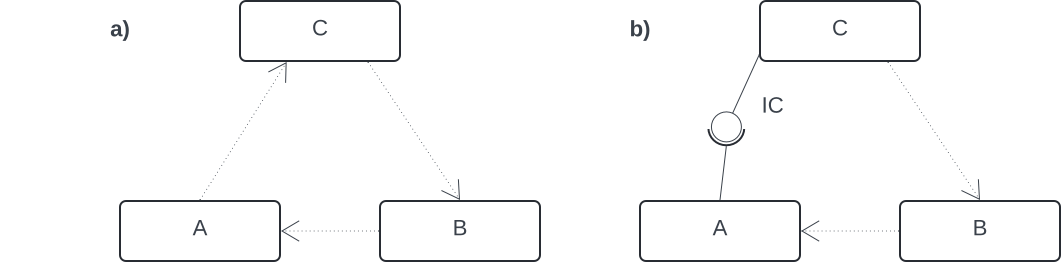
\includegraphics[scale=0.4]{part two/Objektorientierter Entwurf/img/zirkulaer}
    \caption{
        Beispiel für eine zirkuläre Abhängigkeit (a) und deren Auflösung (b).
        (Quelle: in Anlehnung an \cite[76, Abb. 3.19]{Wed09b})
    }
    \label{fig:zirkulaer}
\end{figure}

\subsubsection*{Liskovsches Substitutionsprinzip}
Das \textbf{Ersetzbarkeitsprinzip} wurde bereits im Zusammenhang mit \textbf{Polymorphie} im Abschnitt~\ref{sec:beziehungen-von-klassen} eingeführt.